%%%% Better Poster latex template example v1.0 (2019/04/04)
%%%% GNU General Public License v3.0
%%%% Rafael Bailo
%%%% https://github.com/rafaelbailo/betterposter-latex-template
%%%% 
%%%% Original design from Mike Morrison
%%%% https://twitter.com/mikemorrison

\documentclass[a0paper,fleqn]{betterposter}

%%%% Uncomment the following commands to customise the format

%% Setting the width of columns
% Left column
\setlength{\leftbarwidth}{0.255\paperwidth}
% Right column
\setlength{\rightbarwidth}{0.255\paperwidth}

%% Setting the column margins
% Horizontal margin
%\setlength{\columnmarginvertical}{0.05\paperheight}
% Vertical margin
%\setlength{\columnmarginhorizontal}{0.05\paperheight}
% Horizontal margin for the main column
%\setlength{\maincolumnmarginvertical}{0.15\paperheight}
% Vertical margin for the main column
%\setlength{\maincolumnmarginhorizontal}{0.15\paperheight}

%% Changing font sizes
% Text font
%\renewcommand{\fontsizestandard}{\fontsize{28}{35} \selectfont}
% Main column font
\renewcommand{\fontsizemain}{\fontsize{65}{55} \selectfont}
% Title font
%\renewcommand{\fontsizetitle}{\fontsize{28}{35} \selectfont}
% Author font
%\renewcommand{\fontsizeauthor}{\fontsize{28}{35} \selectfont}
% Section font
%\renewcommand{\fontsizesection}{\fontsize{28}{35} \selectfont}

%% Changing font sizes for a specific text segment
% Place the text inside brackets:
% {\fontsize{28}{35} \selectfont Your text goes here}

%% Changing colours
% Background of side columns
%\renewcommand{\columnbackgroundcolor}{black}
% Font of side columns
%\renewcommand{\columnfontcolor}{gray}
% Background of main column
\definecolor{oxfordblue}{rgb}{0.0, 0.129, 0.278}
\colorlet{lightoxfordblue}{oxfordblue!20}
\renewcommand{\maincolumnbackgroundcolor}{oxfordblue}
%\renewcommand{\maincolumnbackgroundcolor}{theory}
%\renewcommand{\maincolumnbackgroundcolor}{methods}
%\renewcommand{\maincolumnbackgroundcolor}{intervention}
% Font of main column
%\renewcommand{\maincolumnfontcolor}{gray}

\usepackage{booktabs}
\usepackage{microtype}
\usepackage{amsfonts}
\usepackage{amssymb}
\usepackage{tikz}
\usetikzlibrary{positioning,patterns,calc}
\usepackage{array}
\usepackage{siunitx}
\usepackage{pgfplots}
\usepackage{csvsimple}
\usepgfplotslibrary{patchplots}
\usepackage{array}
\usepackage{tikz}
\usepackage{eucal}
%\graphicspath{{Figs/}}
\tikzset{>=latex}
\usetikzlibrary{automata,positioning}
\usepackage{graphicx}
\usepackage[most]{tcolorbox}
\usepackage{etoolbox}
\patchcmd{\thebibliography}{\section*{\refname}}{}{}{}
\usepackage[algo2e,linesnumbered,ruled,lined]{algorithm2e}
\usepackage{multicol}
\usepackage{colortbl}
\newcommand\inner[2]{\langle #1,#2 \rangle}
\begin{document}	
\betterposter{
%%%%%%%% MAIN COLUMN
\maincolumn{
%%%% Main space
\hspace{10mm}
\includegraphics[height=80mm]{img/BirminghamUniversityCrest.png}\hfill

\includegraphics[height=80mm]{img/ox_logo.png}\hspace{10mm}
\vspace{40mm}
\begin{center}
    {\fontsize{115}{100}\selectfont \textbf{Verifying Reinforcement Learning up to Infinity}}\\
    % {\fontsize{90}{100}\selectfont(LCNFQ)}\\
    \vspace{5mm}
    {\fontsize{45}{70}\selectfont Edoardo Bacci, Mirco Giacobbe, Dave Parker}\\
    {\fontsize{45}{70}\selectfont School of Computer Science, University of Birmingham, UK}\\
    {\fontsize{45}{70}\selectfont Computer Science Department, University of Oxford, UK}\\
\end{center}
\vspace{70mm}
\begin{center}
{\fontsize{75}{85}\selectfont "\textbf{Time-unbounded} safety of deep reinforcement learning agents via \textbf{Template-based polyhedra} abstraction"}
\vspace{70mm}\\
\begin{tikzpicture}
\node [inner sep=0pt] at (0,0) {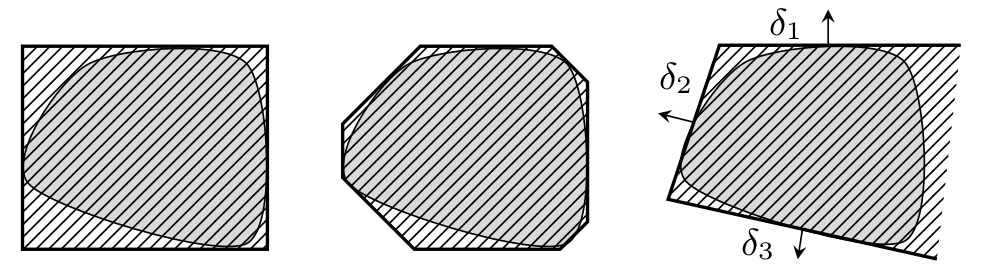
\includegraphics{img/templates.png}};
\draw [white, rounded corners=0.4cm, line width=0.4cm] 
    (current bounding box.north west) -- 
    (current bounding box.north east) --
    (current bounding box.south east) --
    (current bounding box.south west) -- cycle
    ;
\end{tikzpicture}
\end{center}
\vspace{-75mm}
}{
%%%% Bottom space
%% QR code
% points to https://research.birmingham.ac.uk/portal/en/publications/verifying-reinforcement-learning-up-to-infinity(2b0675b2-f13b-4025-aeff-edd83fe83146).html
\begin{center}
\begin{tikzpicture}
\node [inner sep=0pt] at (0,0) {
\includegraphics[height=60mm]{img/qr-code.png}};
\draw [white, rounded corners=0.4cm, line width=0.4cm] 
    (current bounding box.north west) -- 
    (current bounding box.north east) --
    (current bounding box.south east) --
    (current bounding box.south west) -- cycle
    ;
\end{tikzpicture}

\includegraphics[height=45mm]{img/smartphoneWhite}
\\ \textbf{Take a Picture} to Download the Full Paper
% \\ hosein.hasanbeig@cs.ox.ac.uk
% \\ bit.ly/aamas2019
\end{center}
% Smartphone icon
% Author: Freepik
% Retrieved from: https://www.flaticon.com/free-icon/smartphone_65680

%% Compact QR code (comment the previous command and uncomment this one to switch)
%\compactqrcode{img/qrcode}{
%\textbf{Take a picture} to
%\\download the full paper
%}
}

}{
%%%%%%%% LEFT COLUMN
% \title{Logically-Constrained Neural Fitted Q-iteration}
% \author{Mohammadhosein Hasanbeig}
% \author{Alessandro Abate}
% \author{Daniel Kroening}
% \institution{University of Oxford}
\vspace{-5mm}
\begin{tcolorbox}[breakable,colback=white,colframe=oxfordblue,width=\dimexpr\textwidth+12mm\relax,enlarge left by=-6mm,boxrule=3mm,title=\textbf{Introduction},titlerule=5mm,arc=3mm,toptitle=5mm,bottomtitle=5mm,boxsep=5mm]
We introduce the first method for verifying the time-unbounded safety of neural networks controlling dynamical systems. The abstract interpretation method that we use, produces a sound overapproximation of the reach set.

In summary, the algorithm:
\begin{itemize}
\item[\textcolor{oxfordblue}{$\blacktriangleright$}] produces template-based polyhedra by using MILP and interval aritmetic
\item[\textcolor{oxfordblue}{$\blacktriangleright$}] provides stronger safety guarantees than previous time-bounded methods
\item[\textcolor{oxfordblue}{$\blacktriangleright$}] shows whether the agent has generalised beyond the length of its training episode
\item[\textcolor{oxfordblue}{$\blacktriangleright$}] can operate with environments that model observation noise
\end{itemize}
\end{tcolorbox}

\vspace{15mm}
\begin{tcolorbox}[breakable,colback=white,colframe=oxfordblue,width=\dimexpr\textwidth+12mm\relax,enlarge left by=-6mm,boxrule=3mm,title=\textbf{Background},titlerule=5mm,arc=3mm,toptitle=5mm,bottomtitle=5mm,boxsep=5mm]
{\em $\Delta$-polyhedron of $X$}:
\begin{equation}
  \cap \{ \{ x \colon \inner{\delta}{x} \leq \rho_X(\delta)\} \colon \delta \in \Delta \},\label{eq:tpoly}
\end{equation}
where $\rho_X(\delta) = \sup\{ \inner{\delta}{x} \colon x \in X\}$\\
\vspace{7mm}
\textcolor{oxfordblue}{\rule{\textwidth}{3mm}}
The system dynamics are determined by a difference equation 
$$  x_{t} = f(x_{t-1}, a_t) + c_t,\qquad c_t \in C, \qquad x_0 \in X_0$$

where $x_t \in \Real^n$, $a_t \in A$, and $c_t$
respectively denote state, input action, and control
disturbance at time $t$.\\
\vspace{7mm}
\textcolor{oxfordblue}{\rule{\textwidth}{3mm}}
The action of the agent is determined by the neural network controller
$$a_t = \sigma(y_{t-1})$$
\end{tcolorbox}

\vspace{15mm}
\begin{tcolorbox}[breakable,colback=white,colframe=oxfordblue,width=\dimexpr\textwidth+12mm\relax,enlarge left by=-6mm,boxrule=3mm,title=\textbf{Algorithm in Short},titlerule=5mm,arc=3mm,toptitle=5mm,bottomtitle=5mm,boxsep=5mm]
\begin{itemize}
    \item Start with the initial set $X_0$
    \item For each action $a$ compute the successor \\ $X_{t+1} = \post(X_t)$ subject to $\sigma(y) = a$
    \item For a finite $k$, ensure that $X_k \subseteq \cup \{ X_0, \dots, X_{k-1} \}$
    \item The agent is safe if $\cup \{ X_0, \dots, X_k \} \cap B = \emptyset$.
	\end{itemize}
\end{tcolorbox}
}{
%%%%%%%% RIGHT COLUMN
\vspace{-5mm}
\begin{tcolorbox}[breakable,colback=white,colframe=oxfordblue,width=\dimexpr\textwidth+12mm\relax,enlarge left by=-6mm,boxrule=3mm,title=\textbf{Example problem},titlerule=5mm,arc=3mm,toptitle=5mm,bottomtitle=5mm,boxsep=5mm]


\centering
  \begin{tabular}{ccc}
  \begin{tikzpicture}
    \node (lead) at (2,.6) {\reflectbox{
\includegraphics[width=1cm]{img/small-car.png}}};
    \node (ego) at (0,.6) {\reflectbox{
\includegraphics[width=1cm]{img/small-car.png}}};
    \draw (ego) edge[|-|] (lead);
    \node at (0,-.05) {\footnotesize ego};
    \node at (2,0) {\footnotesize lead};
  \end{tikzpicture}
  &\quad&
  \begin{tikzpicture}
    \node (lead) at (1,.6) {\reflectbox{
\includegraphics[width=1cm]{img/small-car.png}}};
    \node (ego) at (0,.6) {\reflectbox{
\includegraphics[width=1cm]{img/small-car.png}}};
    \node at (0,-.05) {\footnotesize ego};
    \node at (1,0) {\footnotesize lead};
    \node at (.43,1.05) {
\includegraphics[width=.5cm]{img/path14.png}};
  \end{tikzpicture}\vspace{-1mm}\\
%   \footnotesize (a) && \footnotesize (b)
  \end{tabular}\\
  \caption{Adaptive cruise control: a good and a bad state.}

\vspace{5mm}
\end{tcolorbox}

\vspace{15mm}
\begin{tcolorbox}[breakable,colback=white,colframe=oxfordblue,width=\dimexpr\textwidth+12mm\relax,enlarge left by=-6mm,boxrule=3mm,title=\textbf{Results},titlerule=5mm,arc=3mm,toptitle=5mm,bottomtitle=5mm,boxsep=5mm]
\setlength{\columnsep}{25mm}
%double column with image on the left and picture on the right
  \begin{tabular}{cc}
    \begin{tikzpicture}
      \begin{axis}
        \addplot graphics [xmin=25,xmax=210,ymin=0,ymax=40]{img/box.png};
      \end{axis}
    \end{tikzpicture}
    & The overapproximation with intervals produce spurious counterxamples \\
    \begin{tikzpicture}
      \begin{axis}
        \addplot graphics [xmin=25,xmax=210,ymin=0,ymax=40]{img/octagon.png};
      \end{axis}
    \end{tikzpicture}
    & The overapproximation with octagons is more precise but fails to find an invariant\\
    \begin{tikzpicture}
      \begin{axis}
        \addplot graphics [xmin=25,xmax=210,ymin=0,ymax=40]{img/template.png};
      \end{axis}
    \end{tikzpicture} 
    & Using a template allows to abstract away unhelpful data and easily find invariants
    \\
  \end{tabular}
%   \caption{Abstract reach sets of a neural network for
%     adaptive cruise control using different templates (Ex.~\ref{ex:abs}).
%     Plots are projected onto vehicles distance (y-axis) and
%     position of lead (x-axis) and constrained within a window, as shown;
%     different colours correspond to different time steps. }
%   \label{fig:abs}
% \end{figure}

\vspace{-5mm}
\textcolor{oxfordblue}{\rule{\textwidth}{3mm}}
\vspace{1mm}
\begin{center}
    

\scalebox{0.77}{
  \begin{tabular}{llrrrr}
    \toprule
    \multicolumn{1}{c}{Env.} &
    \multicolumn{1}{c}{Abs.} &
    \multicolumn{1}{c}{Safe} &
    \multicolumn{1}{c}{Avg} &
    \multicolumn{1}{c}{Avg} &
    \multicolumn{1}{c}{Avg} \\
    &
    &
    &
    \multicolumn{1}{c}{$k$} &
    \multicolumn{1}{c}{poly.} &
    \multicolumn{1}{c}{runtime} \\
    \midrule
    BB & Rect & 11/11 & 237 & 477 & 40s \\
    BB & Oct & 11/11 & 203 & 411 & 47s \\
    ACC ($\epsilon=0$)& Temp & 20/22 & 467 & 610 & 171s \\
    ACC ($\epsilon=.05$) & Temp & 5/22 & 226 & 337 & 124s \\
    CP ($\tau=.001$) & Temp & 4/6 & 27 & 18 & 67s \\
    CP ($\tau=.02$) & Temp & 3/6 & 100 & 125 & 174s \\
    \bottomrule
  \end{tabular}}
\end{center}
\begin{center}
\vspace{5mm}
{\fontsize{25}{45}\selectfont Results for bouncing ball (BB), adaptive cruise control (ACC)\\ and cartpole (CP) environments}
\end{center}
\end{tcolorbox}

\vspace{15mm}
\begin{tcolorbox}[breakable,colback=white,colframe=oxfordblue,width=\dimexpr\textwidth+12mm\relax,enlarge left by=-6mm,boxrule=3mm,title=\textbf{References},titlerule=5mm,arc=3mm,toptitle=5mm,bottomtitle=5mm,boxsep=5mm]
\bibliographystyle{IEEEtran}
\bibliography{biblio}
\end{tcolorbox}

}
\end{document}